% !TEX program = pdflatex
% !BIB program = biber
% !TEX root = main.tex
% openany means no blank pages before chapters
% oneside means no different offset for odd and even pages
% If oneside is use, openany becomes useless.
\documentclass[oneside,12pt,a4paper]{report}

%% This makes the document duplex (suitable for double-sided printing).
%  Comment out bindingoffset=1cm if print on single sided pages. (however this has unintended effect on book class)

\usepackage[left=2cm,right=2cm,top=2cm,bottom=2cm,bindingoffset=1cm]{geometry}

%% Some self-explanatory packages
\usepackage[backref=true, style=alphabetic, backend=biber, url=false, doi=true, isbn=false]{biblatex}
\addbibresource{library.bib}

% Make the references' font size smaller
%\renewcommand*{\bibfont}{\footnotesize}
\DefineBibliographyStrings{english}{%
  backrefpage = {cited on page},
  backrefpages = {cited on pages},
}

\usepackage{comment}
\usepackage{datetime}
\usepackage[font=small,labelfont=bf,justification=centering]{caption}
\usepackage{subcaption}
\usepackage[pdftex,
            hidelinks,
            pdfencoding=auto,
            pdfauthor={Yukio Fukuzawa},
            pdftitle={Computational Methods for Birdsong Analysis}
           ]{hyperref}
\usepackage{lipsum}
\usepackage{todonotes}
\usepackage{setspace}
\usepackage[bottom]{footmisc}
\usepackage[ampersand]{easylist}
\usepackage{amsmath}
\usepackage{nth}
\usepackage{amsfonts}
\usepackage{amssymb}
\usepackage{pdfpages}
\usepackage{fancyhdr}
%\usepackage{pdfpages}
\usepackage{xparse}
\usepackage{afterpage}
\usepackage{mathtools}
\usepackage{forest}
\usepackage{booktabs}  % publication-quality tables
\usepackage{eqparbox}  % sub-align table cells
\usepackage[referable]{threeparttablex}
\usepackage{makecell}
\usepackage{lipsum}
\usepackage{wrapfig}

\usepackage[safe]{tipa}

% To add picture background to a page
\usepackage{eso-pic}

% More control over list items
\usepackage{enumitem}

%% Font typeface
% This typeface looks better
\usepackage{Alegreya}
% Great math font that goes with Alegreya (Asana Math is better if Xelatex or Lualatex is used)
\usepackage{euler}

% This will scramble the text wrapped in \randomize so that it cannot be copied and pasted. Use this to obfuscate email address and other sensitive data.
\usepackage{randtext}

%% For the figures
% Gantt diagrams for the schedule
\usepackage{pgfgantt}
\usepackage{tikz,xcolor}
\usepackage{graphicx}
\graphicspath{{./figures/}}

\usepackage{pgfplots}
% Need this to properly scale the tikz pictures to pagewidth
\usepackage{tikzscale}
% To make Overleaf happy
\pgfplotsset{compat=newest}
% Utilities of the tikz packages
\usetikzlibrary{shapes,arrows,calc,mindmap,shadows,external,positioning,shapes.geometric,arrows.meta}
\usepackage[crop=pdfcrop,cleanup={.tex,.dvi,.ps,.pdf,.log,.bbl,.run.xml,.bcf}]{pstool}

%% This is required for the background image
\usepackage{eso-pic}

% This is needed because XeLatex has no md5 to check for figure update - it will fallback to plain and simple diff anyway. So this is basically to suppress the warning
\usetikzlibrary{external}
\tikzset{external/up to date check=diff}

%% Enable externalisation of the Tikz figures (They will be rendered and saved as PDF for reuse, instead of recompiling each time)
\tikzexternalize

% To rotate a figure landscape and insert it in a portrait page  creating a mess
\newsavebox{\tempbox}

% Suppress the default suffix given to pdf file generated from eps (e.g. if blah.eps is the source then the default generated pdf will be blah-eps-converted-to.pdf)
\usepackage{epstopdf}
\epstopdfsetup{suffix=}

% This will remove the chapter number from section numberings
\renewcommand*\thesection{\arabic{section}}

% This will romanize chapter numbering (e.g. Chapter I instead of Chapter 1)
\renewcommand{\thechapter}{\Roman{chapter}}

% make the chapter title compact
%\usepackage[Glenn]{fncychap}
\usepackage{titlesec, blindtext}
\titleformat{\chapter}[hang]{\LARGE\bfseries}{\thechapter\hspace{20pt}}{0pt}{\LARGE\bfseries}

% This disallows figure numbering to reset after each chapter, so the numbering is continuous throughout the whole document.
\usepackage{chngcntr}
\counterwithout{figure}{chapter}

% For fleuron/dingbats
\usepackage{fourier-orns}

\definecolor{TextColor}{HTML}{000000}
\definecolor{SideColorDark}{HTML}{000000}
\definecolor{MainColor}{HTML}{0000FF}
\definecolor{OppositeColor}{HTML}{FF0000}
\definecolor{HighlightColor}{HTML}{FFFF00}
\color{TextColor}


%% Colour links & citations
\hypersetup{%
  colorlinks=true,
  linkcolor=OppositeColor,
  citecolor=MainColor
}

\makeatletter
\renewcommand*{\p@section}{\S\thechapter-}
\renewcommand*{\p@subsection}{\S\thechapter-\,}
\renewcommand*{\p@subsubsection}{\S\thechapter-}
\renewcommand*{\p@paragraph}{\S\thechapter-}
\makeatother

%% Fancy quote
\usepackage[strict]{changepage}
\usepackage{framed}

\newenvironment{fancyquote}{%
  \def\FrameCommand{%
    \hspace{1pt}%
    {\color{black}\vrule width 2pt}%
    \colorbox{gray!20}%
  }%
  \MakeFramed{\advance\hsize-\width\FrameRestore}%
  \noindent% disable indenting first paragraph
  \begin{adjustwidth}{}{7pt}%
    \vspace{2pt}\vspace{2pt}%
  }
  {%
    \vspace{2pt}\end{adjustwidth}\endMakeFramed%
}

\usepackage{scrextend}

\newcommand{\fncydesc}[2]{
  \begin{fancyquote}
    \begin{labeling}{#1}
      \item[\bfseries\itshape{#1}]\itshape{#2}
    \end{labeling}
  \end{fancyquote}
}

\newcommand{\tudu}[2][]{
  \tikzexternaldisable
    \todo[color=HighlightColor,inline, size=\small,#1]{#2}
  \tikzexternalenable
}

\newcommand{\misfig}[2][]{
  \tikzexternaldisable
  \missingfigure[figcolor=HighlightColor,figwidth=\textwidth,#1]{#2}
  \tikzexternalenable
}

%% Code block style
%  Load the \ttfamily font
\usepackage[T1]{fontenc}
\usepackage[scaled]{beramono}

%  Format code blocks
\usepackage{listings}
%  Change caption name
\renewcommand*{\lstlistingname}{Code block}
\captionsetup[lstlisting]{margin=0cm,format=hang,font=small,format=plain,labelfont={bf,up},textfont={it}}
%  Style
\lstset{
  showstringspaces=false,
  formfeed=\newpage,
  commentstyle=\itshape,
  backgroundcolor=\color{gray!5},
  breakatwhitespace=false,         % sets if automatic breaks should only happen at whitespace
  breaklines=true,                 % sets automatic line breaking
  captionpos=b,                    % sets the caption-position to bottom
  commentstyle=\color{gray},    % comment style
  escapeinside={\%*}{*)},          % if you want to add LaTeX within your code
  keepspaces=true,
  numbersep=2mm,                   % how far the line-numbers are from the code
  showspaces=false,
  showstringspaces=false,
  showtabs=false,
  stepnumber=1, numberfirstline=false,
  basicstyle=\linespread{1}\footnotesize\ttfamily,
  keywordstyle=\bfseries\color{MainColor},
  stringstyle=\itshape\color{OppositeColor},
  numberstyle=\footnotesize\ttfamily\color{gray},
  numbers=left,xleftmargin=4mm,framexleftmargin=0mm,xrightmargin=0mm,
  frame=top,frame=bottom,
}

%% Change title style (currently change only color)
\titleformat{\chapter}
{\normalfont\LARGE\bfseries\color{SideColorDark}}{\thechapter}{1em}{}

\titleformat{\section}
{\normalfont\Large\bfseries\color{SideColorDark}}{\thesection}{1em}{}

\titleformat{\subsection}
{\normalfont\large\bfseries\color{SideColorDark}}{\thesubsection}{1em}{}

\title{VMH FILESYSTEM}
\author{Villon Chen\\
        Moaad Maaroufi\\
        Hamza Jad Al Aoun}
\date{\today}

\doublespacing
\begin{document}
  
  \counterwithout{lstlisting}{chapter}
  \pagenumbering{roman}
  \thispagestyle{empty}
\newgeometry{left=4cm,right=3cm,top=3cm,bottom=2cm}

\begin{titlepage}
  \singlespacing
  \begin{center}
  
    \tikzexternaldisable
    \tikzsetnextfilename{figures/frame}
    \begin{tikzpicture}[overlay, remember picture]
    \draw[-,black,ultra thick]
    ($(current page.north west) + (3cm,-2cm)$) rectangle ($(current page.south east) + (-2cm,2cm)$);
    \draw[-,black,thin]
    ($(current page.north west) + (2.8cm,-2.2cm)$) rectangle ($(current page.south east) + (-1.8cm,2.2cm)$);
    \draw[-,black,thin]
    ($(current page.north west) + (3.2cm,-1.8cm)$) rectangle ($(current page.south east) + (-2.2cm,1.8cm)$);
    \end{tikzpicture}
    \tikzexternalenable
  
    
\includegraphics[height=3cm]{figures/eurecom_logo.jpeg}\\[0.5cm]
  
    % Main title
    \par\vspace{1cm}
    \makeatletter
    \begin{minipage}{\textwidth}
      \centering
      \fontsize{24pt}{24pt}\selectfont\scshape\@title \\[1cm]
      \large Basic OS project\\Fall 2022\\First year engineering program
    \end{minipage}
    \makeatother
    \par\vspace{1.5cm}
    
    \large
    \textbf{BY}\\[0.25cm]
    \makeatletter\@author\makeatother
    \par\vspace{2cm}
    
    {\bfseries{SUPERVISORS}}\\[0.25cm]
    Ludovic Apvrille\\
    Sophie Coudert\\[2cm]
    
    EURECOM Engineering School\\
    Sophia Antipolis, France\\[1cm]
    
    \today
  
  \end{center}
\end{titlepage}
\restoregeometry
  \afterpage{\null\addtocounter{page}{-1}}
  
  %\include{frontmatter/abstract}
  {\hypersetup{linkcolor=black}
    % This allows the paragraphs to be numbered (e.g. 1.2.3.4)
    \setcounter{secnumdepth}{4}
    
    % This allows the TOC to go down to subsection level, but not further
    \setcounter{tocdepth}{3}
    
    \tableofcontents
  }

  \setlength{\parindent}{1em}
  \setlength{\parskip}{0em}

  \pagenumbering{arabic}
  
  % You should always divide your documents into small parts and use \include to merge them together.
  \chapter{Introduction}
\label{cp:introduction}
Usually, when a file system is full, the user gets a "no space left on device" error message: it is not possible to add a new file or extend a file.\\

The objective of the project is to program a new file system that can handle a "no space left on device" error: this new file system we are going to implement assumes that, when the file system is full, the file system deletes the oldest files until it can store the new file.\\

The file system to program is simply an array of data stored as a regular file on the computer. The implementation of files, directories, inodes... and the intuition behind it are going to be discussed thoroughly in the first section.

Six main functions has been implemented in the file system (create, write, read, remove, ls, size) with the objective of reserving as much space as possible for file data. The structure of each one of these functions will be explained in the following sections.
\newpage
  \chapter{File system structure}
\label{cp:file system structure}
As we explained in the introduction, the main characteristic of this file system is the FIFO principle (first in first out) in writing files. So instead of using standard static data blocks, why not use a dynamic queue (FIFO) container which will model perfectly our file system. The cherry on top is that the files in our file system will be always sorted by date (the oldest element is always going to be the first element in the array).\\

In this manner, each time we want to modify the file system we have to put on the RAM, make the necessary modifications and then save it back to the disk. In our case, the size of the file system is just 10 MB, so its not going to affect the RAM. With larger file Systems this approach is obsolete.\\

To do so, we first use a function \textit{get\_FS} that reads a file system stored on the disk to the memory. After the necessary changes are made to the file system, we use the function \textit{put\_FS} that rewrites the file system back into the disk.\\

\begin{table}[hbt!]
    \centering
    \begin{tabular}{|c|}
        \hline
        \textbf{FILESYSTEM} \\
        \hline
        \textbf{SuperBlock sb} \\
        \hline
        \textbf{File * file\_array} \\
        \hline
        \textbf{Directory * directory\_array} \\
        \hline
    \end{tabular}
    \caption{FileSystem structure}
    \label{tab:my_label}
\end{table}

\newpage
In order to facilitate the manipulation of the objects that we are going to use in the file system we chose for our file system to be a \textit{struct} that contains a \textbf{superblock}, a \textbf{directory array} and a \textbf{file array}:

\begin{itemize}
    \item \textbf{The SuperBlock}: which is in itself a \textit{struct} that contains some useful information about the file system(number of files, number of directories, size of the directory array, the current size of the file system, and the maximum size of the file system which is in our case 10 MB).\\

    \begin{table}[hbt!]
        \centering
        \begin{tabular}{|c|}
            \hline
            \textbf{SUPERBLOCK} \\
            \hline
            \textit{long int} file\_number \\
            \textit{long int} directory\_number \\
            \textit{long int} directory\_array\_size \\
            \textit{long int} current\_size \\
            \textit{long int} max\_size \\
            \hline
        \end{tabular}
        \caption{SuperBlock structure}
        \label{tab:my_label}
    \end{table}
    
    \item \textbf{The directory array}: which is an array of structs.
    The directories are going to be modeled by structs that contains its name and the index of its parent directory in the directory array. 
    We chose this implementation so we can link directories to one another easily.
    The root is going to have index zero by convention in its parent id. 
    When we need to remove a particular directory we will just put -1 in its parent id instead of removing it from the directory array(this will mess up the parent child relationship because it relies on the index of each directory in the array and thus changing it will cause problems). 
    In all other implementations, this will taken into account, so by convention parent id = -1 means this directory doesn't exist and we overwrite it with brand new directory.\\

    \begin{table}[hbt!]
        \centering
        \begin{tabular}{|c|}
            \hline
            \textbf{DIRECTORY} \\
            \hline
            \textit{char} name\textit{[WORD\_SIZE]} \\
            \textit{long int} parent\_id \\
            \hline
        \end{tabular}
        \caption{Directory structure}
        \label{tab:my_label}
    \end{table}

    \newpage
    \item \textbf{File array}: which is an array of structs as well, these structs are going to be of type File which is in itself a struct that contains the contents of the file \textit{char* bytes} and another struct named \textit{Inode} which provides some information about the file such as its name, size and its parent directory index.\\

    \begin{table}[hbt!]
        \centering
        \begin{tabular}{|c|}
            \hline
            \textbf{FILE} \\
            \hline
            \textit{Inode} inode \\
            \textit{char *} bytes \\
            \hline
        \end{tabular}
        \caption{File structure}
        \label{tab:my_label}
    \end{table}

    \begin{table}[hbt!]
        \centering
        \begin{tabular}{|c|}
            \hline
            \textbf{INODE} \\
            \hline
            \textit{long int} size\\
            \textit{char} name\textit{[WORD\_SIZE]} \\
            \textit{long int} parent\_id \\
            \hline
        \end{tabular}
        \caption{File structure}
        \label{tab:my_label}
    \end{table}
 
\end{itemize}









\newpage
  \chapter{Commands}

\section{The create command}

\subsection{How it works}
\textbf{\textcolor{blue}{create}}: takes as an input the size of the file system we want to create.\\

When calling the create command, memory will be allocated on the heap for both the directory and the file array since they are dynamic, and then a file system structure is filled with the initial data. Eventually the new file system will have: 
\begin{itemize}
\item max\_size will be size*1000*1000 (size is passed to create in MB and its multiplied by ${10}^{6}$ in order to convert it into bytes).
\item the directory and file's number is initialized to 0.
\item the current size of the file system will updated to the size of the Superblock plus the size of the directory and file arrays.
\item using add\_directory function, root directory "/" with index -2 is added to the file system after allocating memory for 1 Directory struct in the directory array.
\end{itemize}

At the end the FileSystem struct will be stored on the disk using put\_FS function and all the allocated memory will be freed up.

\newpage
\subsection{Testing}
\lstset{language=bash,caption={create command},label=code:create-command}
\begin{lstlisting}
$ vmhFS /tmp/tmpFS create 10
FileSystem created
Size: 80 B
Max size: 10000000 B
Files: 0
Directories: 1
\end{lstlisting}

\lstset{language=bash,caption={File system on the disk},label=code:file-system-on-the-disk}
\begin{lstlisting}
$ stat /tmp/tmpFS 
  File: /tmp/tmpFS
  Size: 10000000        Blocks: 8          IO Block: 4096   regular file
Device: 10302h/66306d   Inode: 5898250     Links: 1
Access: (0664/-rw-rw-r--)  Uid: ( 1000/  michel)   Gid: ( 1000/  michel)
Access: 2022-12-01 14:31:22.790783924 +0100
Modify: 2022-12-01 15:13:15.805815135 +0100
Change: 2022-12-01 15:13:15.805815135 +0100
 Birth: 2022-12-01 13:17:22.874251973 +0100
\end{lstlisting}

\newpage
\section{The ls command}

\subsection{How it works}
\textbf{\textcolor{blue}{ls}}: takes as an input the directory path and two flags: -r for the recursive version and -d to sort the files by date. (By construction of the file system, they're always sorted.)To do its job it uses the following subfunctions:\\

\begin{itemize}
\item \textit {ls\_accumulator(FileSystem fs, long int dir\_id, int level, int max\_level)}: this function is recursive, it takes the directory id as an input, it uses the \textit{get\_dir\_children(fs,id)} function to get all the children directories of the given directory and stores them in a \textit{dir\_children} structure, if the children number of this directory is greater than zero this means that its not empty and has children directories, in this case we will print the name of the directory children and recursively print all the files found in these directories. 
The base condition for this recursive function is \textit{dir\_children.number}==0 i.e to stop when a given directory doesn't have any children directories.\\

\item \textit{Dir\_files get\_dir\_files(FileSystem fs, long int dir\_id)}: this function takes as an input the directory id and find all the files found in this directory.
\end{itemize}
The \textbf{\textcolor{blue}{ls}} function always checks whether the path provided is correct or not. If the recursive flag hasn’t been indicated, it will print the all files inside the desired directory. \\

On the other hand if the recursive flag is present, the ls function prints the files inside the given directory and recursively prints all files  contained in its children directories schemed in a tree representation. \\


\newpage
\subsection{Testing}
\lstset{language=bash,caption={ls command},label=code:ls-command}
\begin{lstlisting}
$ vmhFS /tmp/tmpFS create 10
$ vmhFS /tmp/tmpFS write /tmp/foo.txt /dir1/dir2/dir3/dir4/dir5/foo.txt
$ vmhFS /tmp/tmpFS write /tmp/foo.txt /dir1/foo1.txt
$ vmhFS /tmp/tmpFS write /tmp/foo.txt /dir1/foo2.txt
$ vmhFS /tmp/tmpFS write /tmp/foo.txt /dir1/foo3.txt
$ vmhFS /tmp/tmpFS ls /dir1
$ vmhFS /tmp/tmpFS ls /dir1 -r
\end{lstlisting}

\lstset{language=bash,caption={Command output},label=code:command-output}
\begin{lstlisting}
Write file /tmp/foo.txt to filesystem at: /dir1/dir2/dir3/dir4/dir5/foo.txt
Write file /tmp/foo.txt to filesystem at: /dir1/foo1.txt
Write file /tmp/foo.txt to filesystem at: /dir1/foo2.txt
Write file /tmp/foo.txt to filesystem at: /dir1/foo3.txt
List segment:
dir1
L__foo1.txt [18 B]
L__foo2.txt [18 B]
L__foo3.txt [18 B]
L__dir2
List segment:
dir1
L__foo1.txt [18 B]
L__foo2.txt [18 B]
L__foo3.txt [18 B]
L__dir2
    L__dir3
        L__dir4
            L__dir5
                L__foo.txt [18 B]
\end{lstlisting}

\newpage
\section{The read command}

\subsection{How it works}
\textcolor{blue}{\textbf{read}}: returns the bytes of the file. It takes in argument the path to the file.
First it checks if the path refers to a file and not a directory.\\

Then, we call the function \textit{file\_from\_path}. If it returns a value  equal to -1, that means the file doesn't exist. Else, we'll use the function \textit{file\_id} to get the index of the file in the \textit{file\_array}.\\

Thanks to the File struct, we can access easily to the content of the file with the member \textit{File.bytes}. Finally we print it in the standard output.\\
\begin{center}
    \begin{tabular}{cc}
        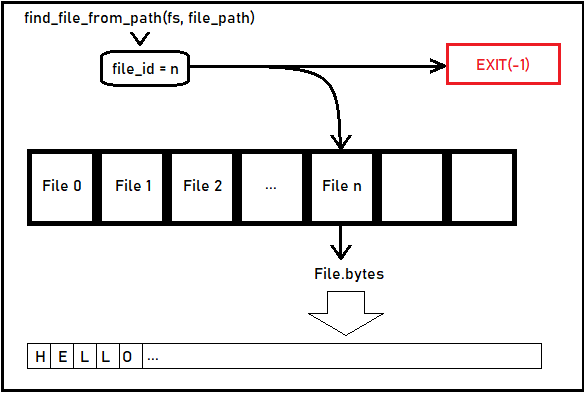
\includegraphics{figures/read.png}
    \end{tabular}
    \captionof{figure}{Reading a file (made with MS Paint)}
\end{center}

\newpage
\subsection{Testing}
\lstset{language=bash,caption={Read command},label=code:read-command}
\begin{lstlisting}
$ echo "Random string 123" > /tmp/foo.txt
$ vmhFS /tmp/tmpFS write /tmp/foo.txt /dir1/dir2/foo.txt
$ vmhFS /tmp/tmpFS read /dir1/dir2/foo.txt
$ vmhFS /tmp/tmpFS read /dir1/dir2/foo2.txt
\end{lstlisting}

\lstset{language=bash,caption={Command output},label=code:command-output}
\begin{lstlisting}
Write file /tmp/foo.txt to filesystem at: /dir1/dir2/foo.txt
Random string 123
File doesn't exist
\end{lstlisting}

\newpage
\section{The remove command}

\subsection{How it works}
\textcolor{blue}{\textbf{remove}}: remove a file or directory at the provided path.\\

As we did in the read function we should also check here whether the path is correct or not. To do so, we can call the functions \textit{find\_file\_from\_path} and \textit{find\_dir\_from\_path}.\\

If the path is valid (i.e. there is something at this path in the file system), then we must get a non -1 value (-1 means the file/dir doesn't exist at this path). Else, if we get return value -1 for both of these functions, the path is not valid.\\

Now that we know whether the path refers to a file or a directory, we just need to call the adapted function to remove it (either \textit{rm\_directory or rm\_file)}. Those functions are file system functions, because they are used in other commands as well.\\

Removing a file is different from removing a directory.
On one hand, removing a file consists of removing the file from the \textit{file\_array} and then shift every other file to fill the gap.
On the other hand, removing a directory consists only of setting up the directory's \textit{parent\_id} to -1 (convention) and name to \textit{TRASHED}.\\

Directories should not be shifted like files, because we need to preserve the parent-child relationship between directories and this information is stored inside in \textit{parent\_id} member and their indices in the \textit{directory\_array}.\\

\begin{center}
    \begin{tabular}{cc}
        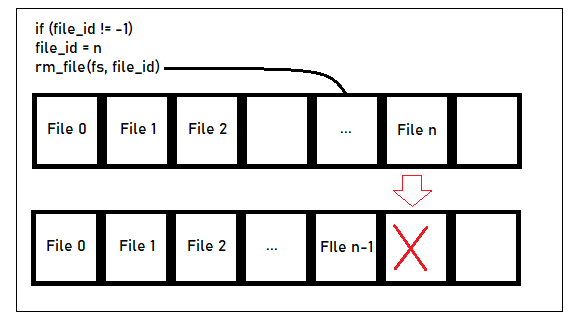
\includegraphics{figures/rm_file.png}
    \end{tabular}
    \captionof{figure}{Removing a file (made with MS Paint)}
\end{center}\\

\begin{center}
    \begin{tabular}{cc}
            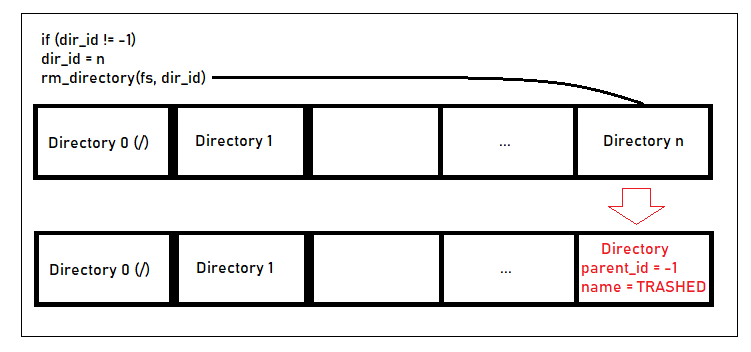
\includegraphics[width=16cm]{figures/rm_directory.png}
    \end{tabular}
    \captionof{figure}{Removing a directory (made with MS Paint)}
\end{center}\\

\newpage
\subsection{Testing}
\lstset{language=bash,caption={Remove command},label=code:remove-command}
\begin{lstlisting}
$ vmhFS /tmp/tmpFS write /tmp/foo.txt /dir1/dir2/foo.txt
$ vmhFS /tmp/tmpFS remove /dir1/dir2/foo.txt
$ vmhFS /tmp/tmpFS remove /dir1/dir2
$ vmhFS /tmp/tmpFS remove /dir1
$ vmhFS /tmp/tmpFS ls / -r
$ vmhFS /tmp/tmpFS remove /
\end{lstlisting}

\lstset{language=bash,caption={Command output},label=code:command-output}
\begin{lstlisting}
Write file /tmp/foo.txt to filesystem at: /dir1/dir2/foo.txt
File /dir1/dir2/foo.txt has been remove from the file system
Directory /dir1/dir2 has been remove from the file system
Directory /dir1 has been remove from the file system
List segment:
/
Root directory cannot be removed
\end{lstlisting}

\newpage

\section{The write command}

\subsection{How it works}
\textit{\textcolor{blue}{\textbf{write}}}: takes as an argument an input file stored in the computer and writes at a specified \textit{destination\_path}.\\

We start with some error handling: we check if the given file exists already in the file system by using the function \textit{find\_file\_from\_path}. This function returns -1 if the file doesn't exist otherwise it returns the index of the file in the file array.\\

After this step we use the function \textit{create\_dir\_from\_path} to check whether the path exists or not, if it does the function proceeds without changing anything. If it doesn't exist or its missing some directories it creates them. \\

Next, we create a struct of type File where we put the content of the input file and the information related to it thanks to the function \textit{get\_file}. Before proceeding we check if the size of the file doesn't exceed 5MB.\\

Now, to add the File struct that we just created to the file system we need to check first if the number of bytes of the file plus the size of one inode can fit in the current file system. If it is the case we add it directly using the function \textit{add\_file}. This function first checks if the file array is empty,if it is we use the the LibC function \textit{malloc} to allocate space for the new file. If there are already some files in the file system, we use \textit{realloc} to allocate more space for the new file. We treated the first case separately to avoid using \textit{realloc} on an empty array as it can result in some memory problems. \\
\newpage

Moving on to the second case now where there isn't enough space to store the new file. Here we should proceed using the FIFO principle.
The first case is where the file array contains only one file, we shall remove it using the function \textit{remove\_file} that we discussed earlier in the remove command. Next, we add it to the file system using  the function \textit{add\_file}. We treat this case separately to avoid using the \textit{realloc} on on empty array. In the second case the file system contains at least two files, we go into a while loop that counts the number of files to be removed from the file system starting from the oldest , in order for our new file to fit.\\

Now we should shift the files to the left in the file array by the number of files that should be removed (that we counted earlier with the while loop). Afterwards we reallocate the file array to fit the current number of files. Eventually we add the new file at end of the file array.

\subsection{Testing}
\lstset{language=bash,caption={Write command},label=code:write-command}
\begin{lstlisting}
$ vmhFS /tmp/tmpFS write /tmp/4mb /dir1/dir2/4mb1
$ vmhFS /tmp/tmpFS write /tmp/4mb /dir1/dir2/4mb2
$ vmhFS /tmp/tmpFS write /tmp/4mb /dir1/dir2/4mb3
$ vmhFS /tmp/tmpFS ls / -r
\end{lstlisting}

\lstset{language=bash,caption={Command output},label=code:command-output}
\begin{lstlisting}
Write file /tmp/4mb to filesystem at: /dir1/dir2/4mb1
Write file /tmp/4mb to filesystem at: /dir1/dir2/4mb2
Write file /tmp/4mb to filesystem at: /dir1/dir2/4mb3
List segment:
/
L__dir1
    L__dir2
        L__4mb2 [4194304 B]
        L__4mb3 [4194304 B]
\end{lstlisting}

\newpage

\section{The size command}

\subsection{How it works}
\textcolor{blue}{\textbf{size}}: computes the size of files inside a given directory. If the -r flag is indicated, size should recursively calculate the size of files inside that directory. \\

This function takes as an argument the directory path. We use the function \textit{find\_dir\_from\_path} to check if the path is correct, if not it returns -1. If the path exists indeed, it returns the directory index in the directory file.\\

We also use the function \textit{size\_dir\_files} that calculates the size of files inside a single directory with a simple for loop over the file array.\\

For the recursive part, we use the function \textit{size\_accumulator} that takes in argument an index of a given directory. The base condition of this recursive function is to stop at a directory that doesn't have any children directories. We compute the indices of a given directory by using the function \textit{get\_dir\_children} that uses another simple for loop over the directory array. Its algorithm is very similar to the one used in the recursive ls.\\

\newpage
\subsection{Testing}
\lstset{language=bash,caption={Size command},label=code:size-command}
\begin{lstlisting}
$ vmhFS /tmp/tmpFS write /tmp/foo.txt /dir1/foo1.txt
$ vmhFS /tmp/tmpFS write /tmp/4mb /dir2/4mb1
$ vmhFS /tmp/tmpFS size /dir1 -b -r
$ vmhFS /tmp/tmpFS size /dir2 -k -r
$ vmhFS /tmp/tmpFS size / -b -stat
\end{lstlisting}

\lstset{language=bash,caption={Command output},label=code:command-output}
\begin{lstlisting}
Write file /tmp/4mb to filesystem at: /dir1/dir2/4mb1
Write file /tmp/4mb to filesystem at: /dir1/dir2/4mb2
Write file /tmp/4mb to filesystem at: /dir1/dir2/4mb3
List segment:
/
L__dir1
    L__dir2
        L__4mb2 [4194304 B]
        L__4mb3 [4194304 B]
Write file /tmp/foo.txt to filesystem at: /dir1/foo1.txt
Write file /tmp/4mb to filesystem at: /dir2/4mb1
Total size of files in /dir1: 18 B [Recursive]
Total size of files in /dir2: 4194 KB [Recursive]
Current size of the file system 12583532
Total size of the files: 4194322
Ratio Total files/Total filesystem: 0.33332
Total size of files in /: 0 B [Not recursive]
\end{lstlisting}

\newpage



  \chapter{Conclusion}
\label{cp:conclusion}

All the VMH File system commands work as expected and fulfill the initial requirements. The queue structure of the file system simplified the implementation of the other functions. Furthermore, the advantage of working on the RAM is that we make one load and one save instead of repeating this process multiple times for each micro-modification if we were to have a static structure on the disk.
But this approach will only work for very small file systems as mentioned before. To counter this problem, a possible solution is to segment the file system and load it into the RAM segment by segment to make the necessary modifications.We could also add a recursive flag to the remove command, the implementation is going to be similar to the ls and size commands.

\end{document}

